\subsection{Extension}
\begin{namedframe}{Secant and tangents}
	\begin{columns}
		\begin{column}{0.5\textwidth}
			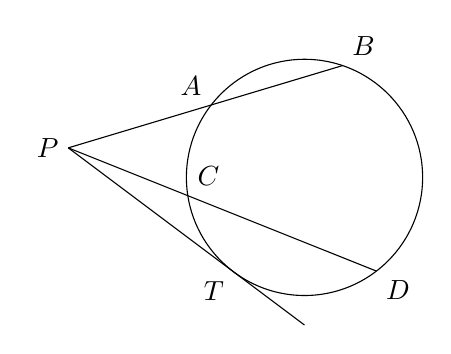
\begin{tikzpicture}[scale=0.3]
				\coordinate (O) at (0,0);
				\coordinate [label=left:$P$](P) at (-10,1.25);
				\coordinate [label=below left:$T$](T) at (-3,-4);
				\coordinate (E) at (0,-6.25);

				\coordinate [label=above left:$A$](A) at (-3.951,3.065);
				\coordinate [label=above right:$B$](B) at (1.611,4.733);
				\coordinate [label=above right:$C$](C) at (-4.94,-0.774);
				\coordinate [label=below right:$D$](D) at (3.043,-3.967);

				\draw (O) circle (5);
				\draw (P) -- (A) -- (B);
				\draw (P) -- (C) -- (D);
				\draw (P) -- (T) -- (E);
			\end{tikzpicture}
		\end{column}
		\begin{column}{0.5\textwidth}
			\pause
			\begin{example}
				In the diagram $PAB$ and $PCD$ are two secants of the same circle and they intersect at a point $P$ outside the circle.
				\sep
				Prove that $(PA)(PB) = (PC)(PD)$.
				\pause
				This proof also uses similar triangles.
				Try it yourself!
			\end{example}
		\end{column}
	\end{columns}
	\pause
	\begin{example}
		If $PT$ is a tangent to the circle, prove that $(PA)(PB) = (PT)^2$.
	\end{example}
\end{namedframe}
